\subsection{Venezuela}\label{subsec:ven}

LAGO-Venezuela has one operative WCD located in M\'erida City, Universidad de
Los Andes (Merida-ULA), another non operative WCD located in Caracas City,
Universidad Sim\'on Bolivar, (Caracas-USB), and one planned WCD also in
Caracas, Universidad Central de Venezuela, (Caracas-UCV).

Merida-ULA and Caracas-USB have equal electronics: Nexys2 Spartan-3E FPGA
Board, LAGO signal Analog-to-digital converter, switched power source and GPS.
ULA uses one 5' PMT and USB uses one 9' PMT. 

Caracas-USB recently acquired a new Nexys2 in order to restart his wcd
operation. Caracas-UCV has planned to acquire his wcd equipment in the next
semester period, until march of 2014.

There is a plastic WCD of 1\,m height and 76\,cm of diameter. In figure
\ref{fig:wcd-ven} it is shown a photo of the detector. %no hay una foto
mejor del detector? en la que se vea algo de como es?
 
\begin{figure}[htp!]
\centering
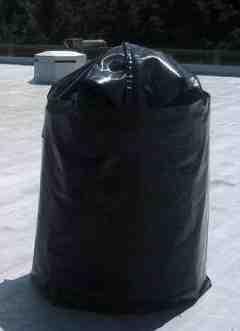
\includegraphics[width=0.30\textwidth,height=0.2\textheight]{images/venezuela/hugo.jpg}
\caption{One of the WCD of the Venezuela LAGO site, called Hugo.}
\label{fig:wcd-ven}
\end{figure}  

Se cuenta con un fotomultiplicador de 5 pulgadas con su divisor de Voltaje,
cuyo diseño fue suministrado por la colaboración LAGO- Perú. Este
fotomultiplicador esta en procesos de pruebas, lo que se ha obetido hasta ahora
es el pulso mostrado en figura 7
  
 \begin{figure}[htp!]
     \centering
     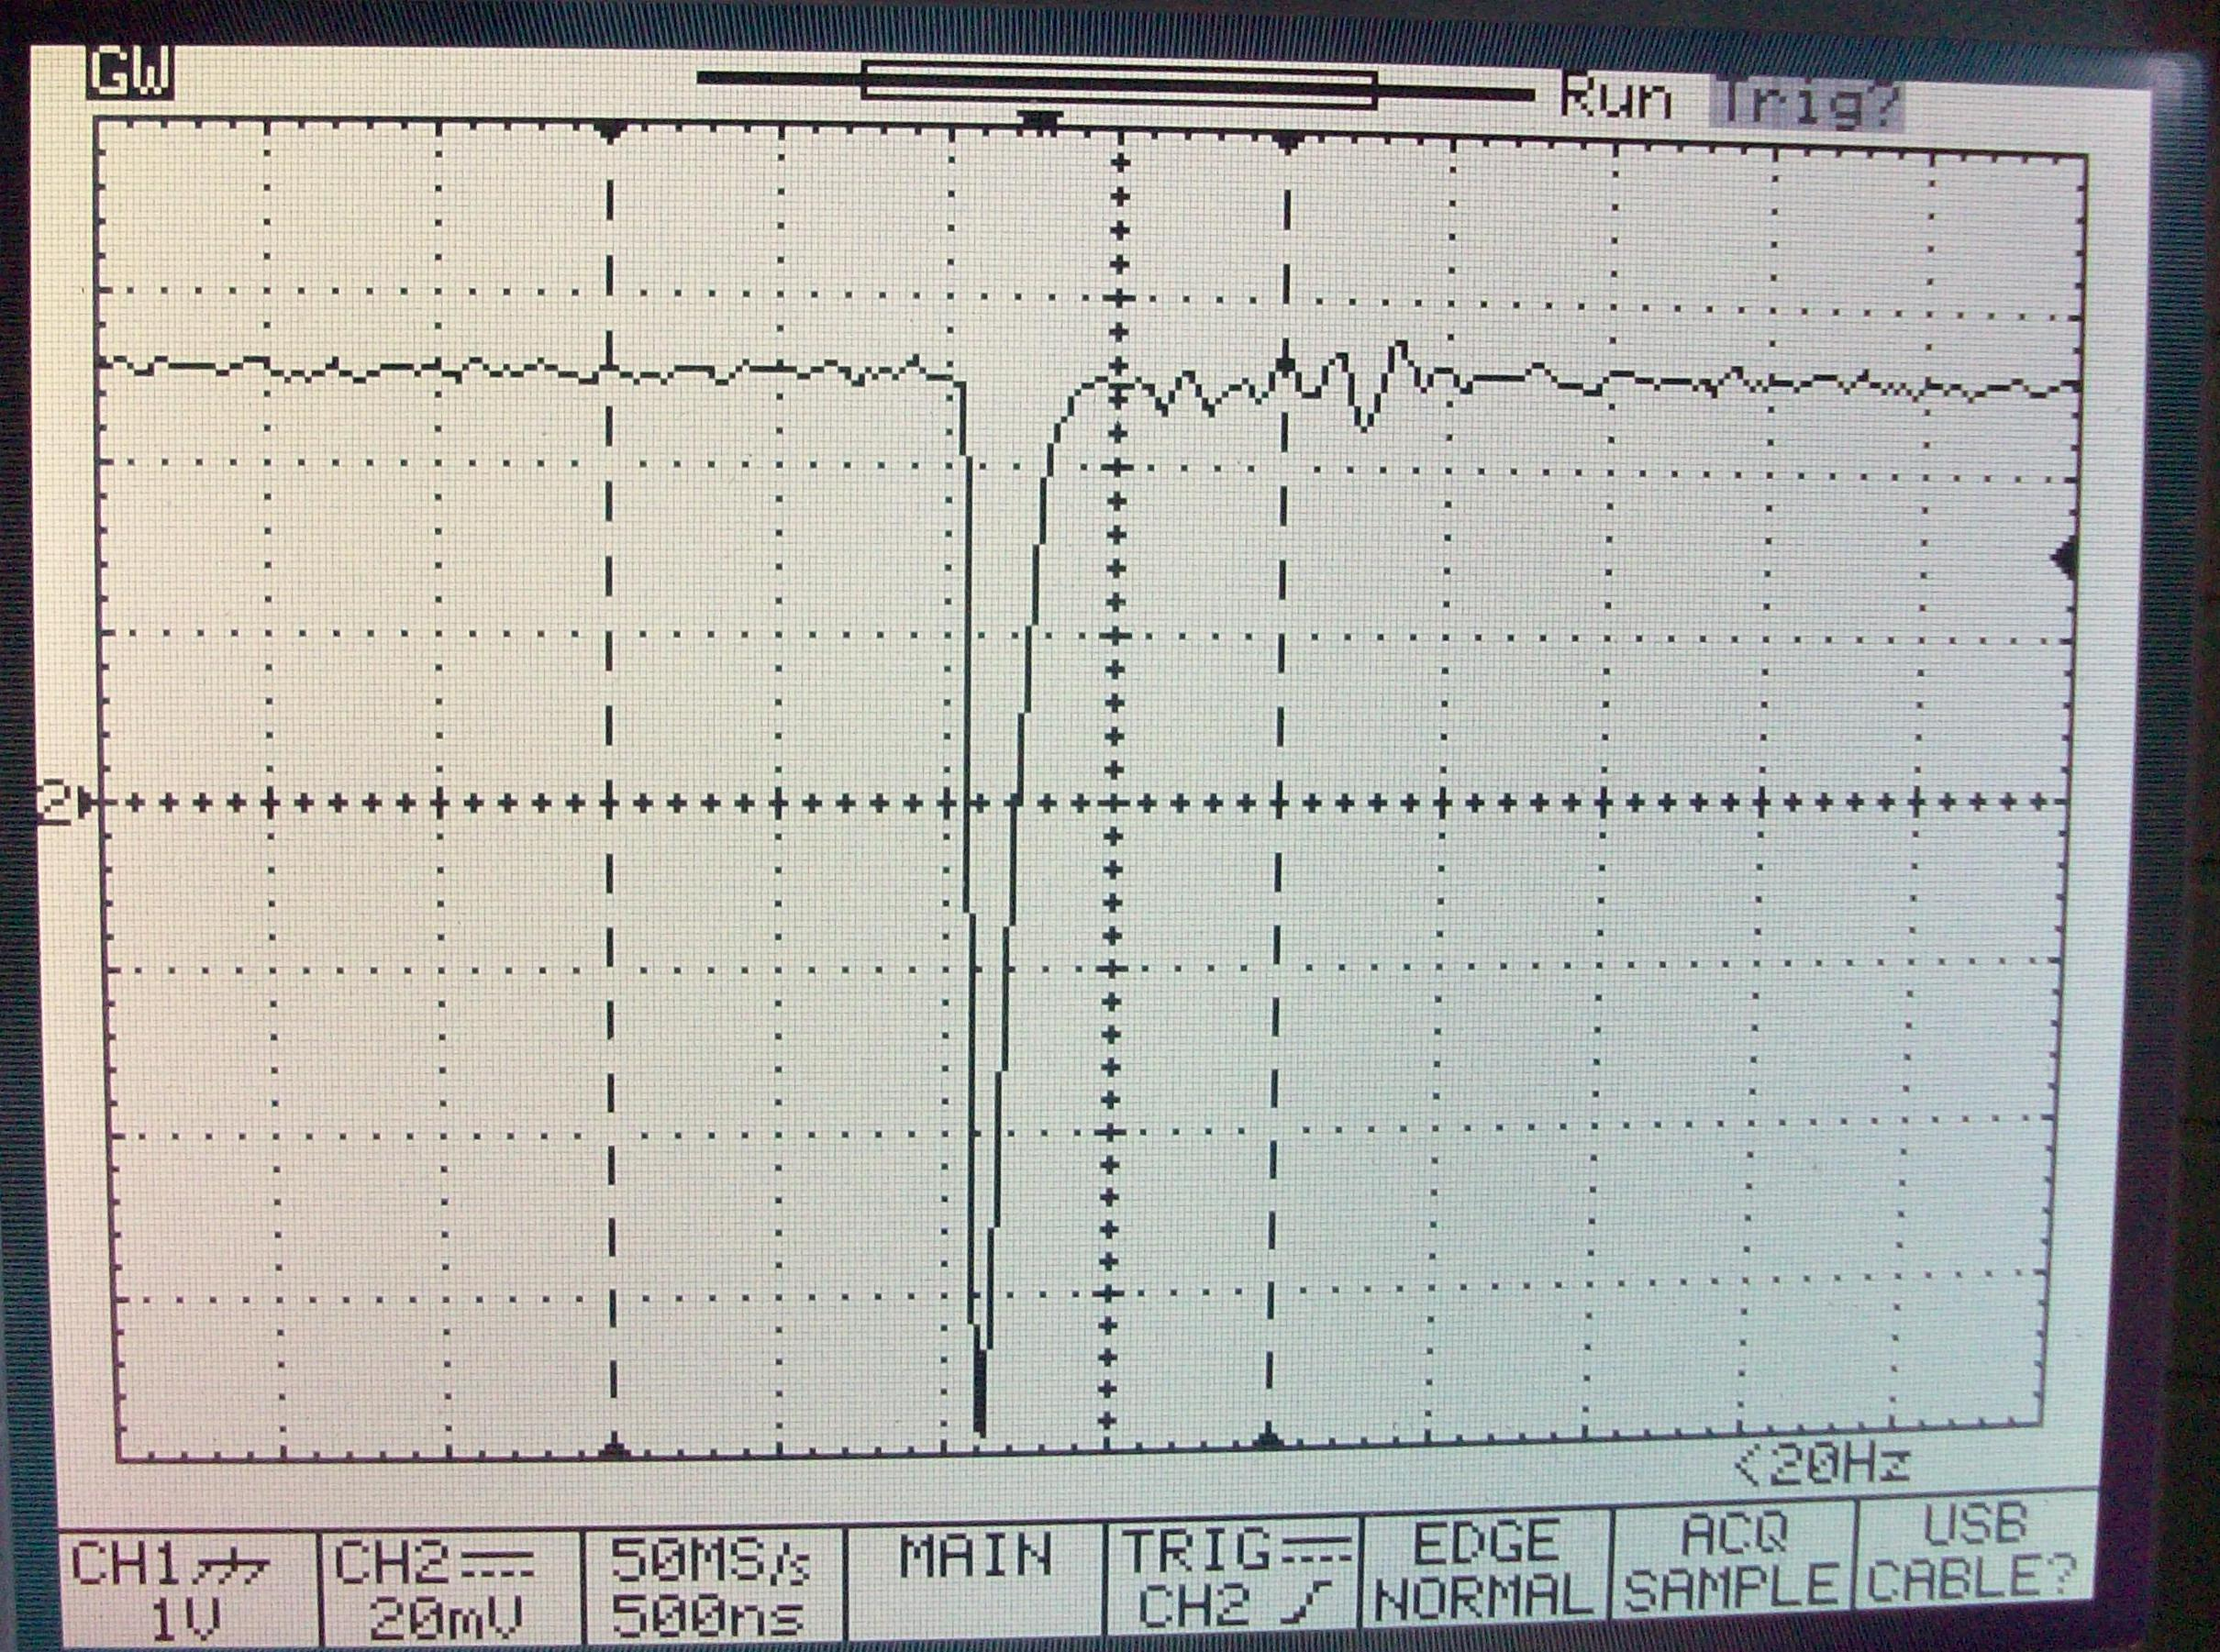
\includegraphics[width=0.65\textwidth,height=0.30\textheight]{images/venezuela/pulsopmt.jpg}
      % nexys2.jpeg: 231x218 pixel, 72dpi, 8.15x7.69 cm, bb=0 0 231 218
     \caption{Pulso con el Fotomultiplicador Pequeño con un Voltaje de $\sim 1800V$} 
     \end{figure}  
 
  
